 
\begin{DoxyImageNoCaption}
  \mbox{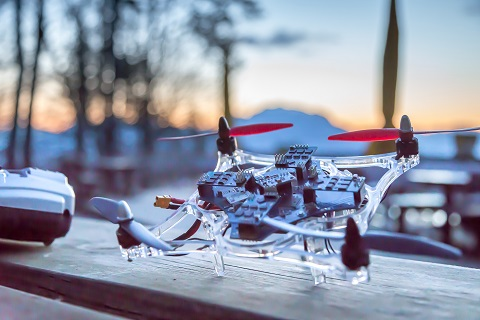
\includegraphics[width=\textwidth,height=\textheight/2,keepaspectratio=true]{QuadroMainpage.jpg}}
\end{DoxyImageNoCaption}


The L\+A\+R\+IX Flight-\/\+Controller is the Flight-\/\+Controller software for the L\+A\+R\+IX Quadrocopter Demonstrator.~\newline
 Built on top the D\+A\+V\+E4 Apps and X\+MC library it provides an easy to configure solution which can be easily modified.~\newline
\hypertarget{index_support}{}\section{Supported devices and toolchains}\label{index_support}
The following 32-\/\+Bit Industrial Microcontrollers based on A\+RM Cortex-\/\+M4F are supported\+:
\begin{DoxyItemize}
\item X\+M\+C4500 series
\end{DoxyItemize}

The following tool chains are supported\+:
\begin{DoxyItemize}
\item G\+NU G\+CC for A\+RM (gcc) found in D\+A\+V\+E4.
\end{DoxyItemize}\hypertarget{index_overview}{}\section{Overview}\label{index_overview}
Main function of this piece of software is to collect the data of the user input\+:
\begin{DoxyItemize}
\item Bluetooth (R\+N42) or
\item R\+C-\/\+Receiver (D\+S\+M\+X-\/\+Spektrum) ~\newline

\end{DoxyItemize}

and the internal sensors\+:
\begin{DoxyItemize}
\item M\+P\+U9\+X50 (Inertial Measurement Unit)
\item D\+P\+S310 (Precision pressure sensor)
\end{DoxyItemize}

to calculate and transmit needed speed of motors so that a stable flight is ensured. ~\newline


The L\+A\+R\+I\+X-\/\+Flight Controller Software consists of several files all stored at the \+\_\+\+Quadrocopter folder. ~\newline
 Within this \+\_\+\+Quadrocopter folder you find several subfolders, which represent nearly independent modules ~\newline
 that are built on top of D\+A\+V\+E4 Apps, the X\+MC Library and a rudimentary Harware Abstraction Layer. ~\newline


The software is interrupt driven which means every sensor and the control interrupt is caused by ~\newline
 it\textquotesingle{}s individual interrupt source which could be a timer or an external interrupt that is triggered by the ~\newline
 sensor itself. Detailed information for each Interrupt and the corresponding service routine can be found at the~\newline
 end of this document. ~\newline


A debug interface is given via uC Probe\+: \href{http://www.infineon.com/cms/de/product/microcontroller/development-tools-software-and-kits/dave-version-4-free-development-platform-for-code-generation/uc-probe-xmc-for-industrial-mcu/channel.html?channel=5546d46254e133b40154f34038fe1620#ispnTab1}{\tt uC Probe} ~\newline
 or via a V\+C\+OM Port provided by a U\+SB interface which is configured and used via U\+S\+B\+\_\+\+V\+C\+OM App.

More details on hard-\/ and software of the L\+A\+R\+IX Quadrocopter Demonstrator can be found at\+:
\begin{DoxyItemize}
\item \href{https://github.com/ManagementCenterInnsbruck/InfineonMulticopter_LARIX/wiki}{\tt https\+://github.\+com/\+Management\+Center\+Innsbruck/\+Infineon\+Multicopter\+\_\+\+L\+A\+R\+I\+X/wiki}
\item \href{http://www.infineon.com/cms/en/applications/consumer/multicopters/}{\tt http\+://www.\+infineon.\+com/cms/en/applications/consumer/multicopters/}
\end{DoxyItemize}\hypertarget{index_moduleDescription}{}\section{Module Description}\label{index_moduleDescription}
{\bfseries  Folder Structure\+: }  
\begin{DoxyImageNoCaption}
  \mbox{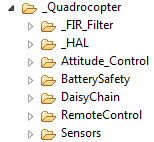
\includegraphics[width=\textwidth,height=\textheight/2,keepaspectratio=true]{FolderStructure.PNG}}
\end{DoxyImageNoCaption}



\begin{DoxyItemize}
\item \+\_\+\+F\+I\+R\+\_\+\+Filter~\newline
 This module provides a simple implementation of a finite impulse response filter. ~\newline
 It is used for filtering the pressure data provided by the D\+P\+S310.
\item \+\_\+\+H\+AL~\newline
 This module builds the basis for serial communication via~\newline
 U\+A\+RT and I2C and holds the files for a delay function.~\newline
 In addition it contains the file G\+P\+I\+O.\+h which provides an easy way to control~\newline
 the digital pins of the controller.
\item Attitude\+\_\+\+Control~\newline
 This module holds the control algorithms for the Quadrocopter.~\newline
 In addition it contains the function for scaling the output values of the control algorithm to the input values of the electric speed controllers(E\+SC\textquotesingle{}s).~\newline

\item Battery\+Safety~\newline
 This module contains the software for battery monitoring.~\newline
 It shows battery status via three status L\+ED\textquotesingle{}s that are mounted at~\newline
 the L\+A\+R\+IX board.
\item Daisy\+Chain~\newline
 This module provides functions to transmit data using an U\+A\+RT Daisy\+Chain which connects the flight controller~\newline
 with the E\+SC\textquotesingle{}s. The possibility to add feedback data from the E\+SC\textquotesingle{}s is given, but is not implemented.
\item Remote\+Control~\newline
 This module contains the software for receiving the steering data of the user.~\newline
 The two supported ways of communication are Bluetooth(R\+N-\/42 module)~\newline
 and 2.\+4\+G\+Hz Radio(\+Spektrum D\+S\+M\+X Receiver, Spektrum D\+X6i transmitter).~\newline
 A Bluetooth-\/\+Only mode can be configured via a \#define at the \hyperlink{_r_c_receive_8h}{R\+C\+Receive.\+h}
\item Sensors~\newline
 This module contains the software for configuring, reading and interpreting the~\newline
 values of both the D\+P\+S310 pressure sensor and the M\+P\+U9\+X50 Inertial Measurement Unit(\+I\+M\+U). Both are signaling new values~\newline
 by triggering external interrupts.
\end{DoxyItemize}\hypertarget{index_interrupts}{}\section{Interrupts at L\+A\+R\+I\+X Flight-\/\+Controller software}\label{index_interrupts}
Like described at the section overview the L\+A\+R\+IX Flight-\/\+Controller software~\newline
 is an interrupt driven software. This means a set of functions exists, which are executed when~\newline
 a specific event triggers an interrupt.~\newline
 It is important to know that these functions can be interrupted by each other depending on their~\newline
 priority. Priority 0 is the highest priority while 63 is the last priority that can be given~\newline
 to an interrupt function.~\newline
 At Dave4 Interrupts are handled via I\+N\+T\+E\+R\+R\+U\+PT App.~\newline


L\+A\+R\+IX Flight-\/\+Controller software uses global variables to communicate with other interrupt routines.~\newline
 It is important to note that every variable, which is used by more than one interrupt is only allowed to be directly~\newline
 manipulated by one interrupt. Every other interrupt which wants to use the data stored at these globals~\newline
 has to make a local copy of the global one. This is done to avoid unwanted change of global variables~\newline
 which would influence stability of the other software modules.

The next table shows all independent interrupt routines and their purpose. ~\newline


\hypertarget{index_multi_row}{}
\tabulinesep=1mm
\begin{longtabu} spread 0pt [c]{*6{|X[-1]}|}
\caption{Interrupt Overview}\label{index_multi_row}\\
\hline
\rowcolor{\tableheadbgcolor}{\bf Number }&{\bf Interrupt Service Routine }&{\bf Priority }&{\bf Event }&{\bf Description }&{\bf Found at }\\\cline{1-6}
\endfirsthead
\hline
\endfoot
\hline
\rowcolor{\tableheadbgcolor}{\bf Number }&{\bf Interrupt Service Routine }&{\bf Priority }&{\bf Event }&{\bf Description }&{\bf Found at }\\\cline{1-6}
\endhead
\rowcolor{\tableheadbgcolor}{\bf 1 }&{\bf Util\+\_\+\+Timer\+\_\+\+I\+SR }&{\bf 2 }&{\bf Triggered by Utils\+\_\+\+Timer(1 k\+Hz) }&{\bf Builds the basis of delay function }&{\bf ./\+\_\+\+H\+A\+L/\+Delay/util.c }\\\cline{1-6}
\rowcolor{\tableheadbgcolor}{\bf 2 }&{\bf Control\+\_\+\+Timer\+\_\+\+I\+SR }&{\bf 5 }&{\bf Triggered by Control\+\_\+\+Timer(100 Hz) }&{\bf Contains the Control Algorithm for Quadcopter }&{\bf ./\+Attitude\+\_\+\+Control/\+Attitude\+Controller.c }\\\cline{1-6}
\rowcolor{\tableheadbgcolor}{\bf 3 }&{\bf Remote\+Control\+\_\+\+R\+X\+\_\+\+I\+SR }&{\bf 7 }&{\bf 32 Bytes of data are received at U\+A\+RT for RC }&{\bf Data gets read out and interpreted to new desired values }&{\bf ./\+Remote\+Control/\+R\+C\+Receive.c }\\\cline{1-6}
\rowcolor{\tableheadbgcolor}{\bf 4 }&{\bf Bluetooth\+\_\+\+R\+X\+\_\+\+I\+SR }&{\bf 8 }&{\bf 19 Bytes of data are received at U\+A\+RT for Bluetooth }&{\bf Data gets read out and interpreted to new desired values }&{\bf ./\+Remote\+Control/\+R\+C\+Receive.c }\\\cline{1-6}
\rowcolor{\tableheadbgcolor}{\bf 5 }&{\bf M\+P\+U9\+X50\+\_\+\+Ext\+\_\+\+Int\+\_\+\+I\+SR }&{\bf 10 }&{\bf Rising Edge on P0.\+5 detected }&{\bf Data gets read and new orientation is calculated }&{\bf ./\+Sensors/\+M\+P\+U9\+X50/\+M\+P\+U9150.c }\\\cline{1-6}
\rowcolor{\tableheadbgcolor}{\bf 6 }&{\bf D\+P\+S310\+\_\+\+E\+X\+T\+\_\+\+I\+N\+T\+\_\+\+I\+SR }&{\bf 12 }&{\bf Falling Edge on P1.\+15 detected }&{\bf Data gets read out and interpreted to new pressure value }&{\bf ./\+Sensors/\+D\+P\+S310/\+D\+P\+S310.c }\\\cline{1-6}
\rowcolor{\tableheadbgcolor}{\bf 7 }&{\bf Watch\+RC }&{\bf 17 }&{\bf Triggered by RC Watch Timer(5 Hz) }&{\bf check if new value from RC or Bluetooth -\/$>$ timeoutflag }&{\bf ./\+Remote\+Control/\+R\+C\+Receive.c }\\\cline{1-6}
\rowcolor{\tableheadbgcolor}{\bf 8 }&{\bf General\+Purpose\+\_\+\+Timer\+\_\+\+Bluetooth\+\_\+\+Keep\+\_\+\+Alive\+\_\+\+I\+SR }&{\bf 20 }&{\bf Triggered by General Purpose Timer(1 Hz) }&{\bf Sends keep alive message for Android app }&{\bf ./\+Remote\+Control/\+R\+C\+Receive.c }\\\cline{1-6}
\rowcolor{\tableheadbgcolor}{\bf 9 }&{\bf V\+Bat\+\_\+\+Measurement\+\_\+\+I\+SR }&{\bf 30 }&{\bf A\+DC Conversion of Battery Voltage finished }&{\bf Voltage is read out of register and displayed trough L\+E\+Ds }&{\bf ./\+Battery\+Safety/\+Battery\+Safety.c }\\\cline{1-6}
\rowcolor{\tableheadbgcolor}{\bf 10 }&{\bf Magnetometer\+Cal\+\_\+\+Timer\+\_\+\+I\+SR }&{\bf 63 }&{\bf Triggered by Magnetometer\+Cal\+\_\+\+Timer(10 Hz) }&{\bf Not implemented }&{\bf $\ast$\+\_\+\+\_\+\+\_\+\+\_\+\+\_\+\+\_\+\+\_\+\+\_\+\+\_\+\+\_\+\+\_\+\+\_\+\+\_\+\+\_\+\+\_\+\+\_\+\+\_\+\+\_\+\+\_\+\+\_\+\+\_\+\+\_\+\+\_\+\+\_\+\+\_\+\+\_\+\+\_\+\+\_\+\+\_\+\+\_\+\+\_\+$\ast$ }\\\cline{1-6}
\rowcolor{\tableheadbgcolor}{\bf 11 }&{\bf Daisy\+Chain\+\_\+\+R\+X\+\_\+\+I\+SR }&{\bf 63 }&{\bf should be triggered when 13\+Bytes of Data are received at Daisy Uart }&{\bf Not implemented }&{\bf $\ast$\+\_\+\+\_\+\+\_\+\+\_\+\+\_\+\+\_\+\+\_\+\+\_\+\+\_\+\+\_\+\+\_\+\+\_\+\+\_\+\+\_\+\+\_\+\+\_\+\+\_\+\+\_\+\+\_\+\+\_\+\+\_\+\+\_\+\+\_\+\+\_\+\+\_\+\+\_\+\+\_\+\+\_\+\+\_\+\+\_\+\+\_\+$\ast$ }\\\cline{1-6}
\end{longtabu}
~\newline


To give a better overview of this table the image under this text was created.~\newline
 Keep in mind that this picture\textquotesingle{}s purpose is to give an overview but not an exact representation of~\newline
 the Software.~\newline


{\bfseries Simple Flow-\/\+Chart}


\begin{DoxyImageNoCaption}
  \mbox{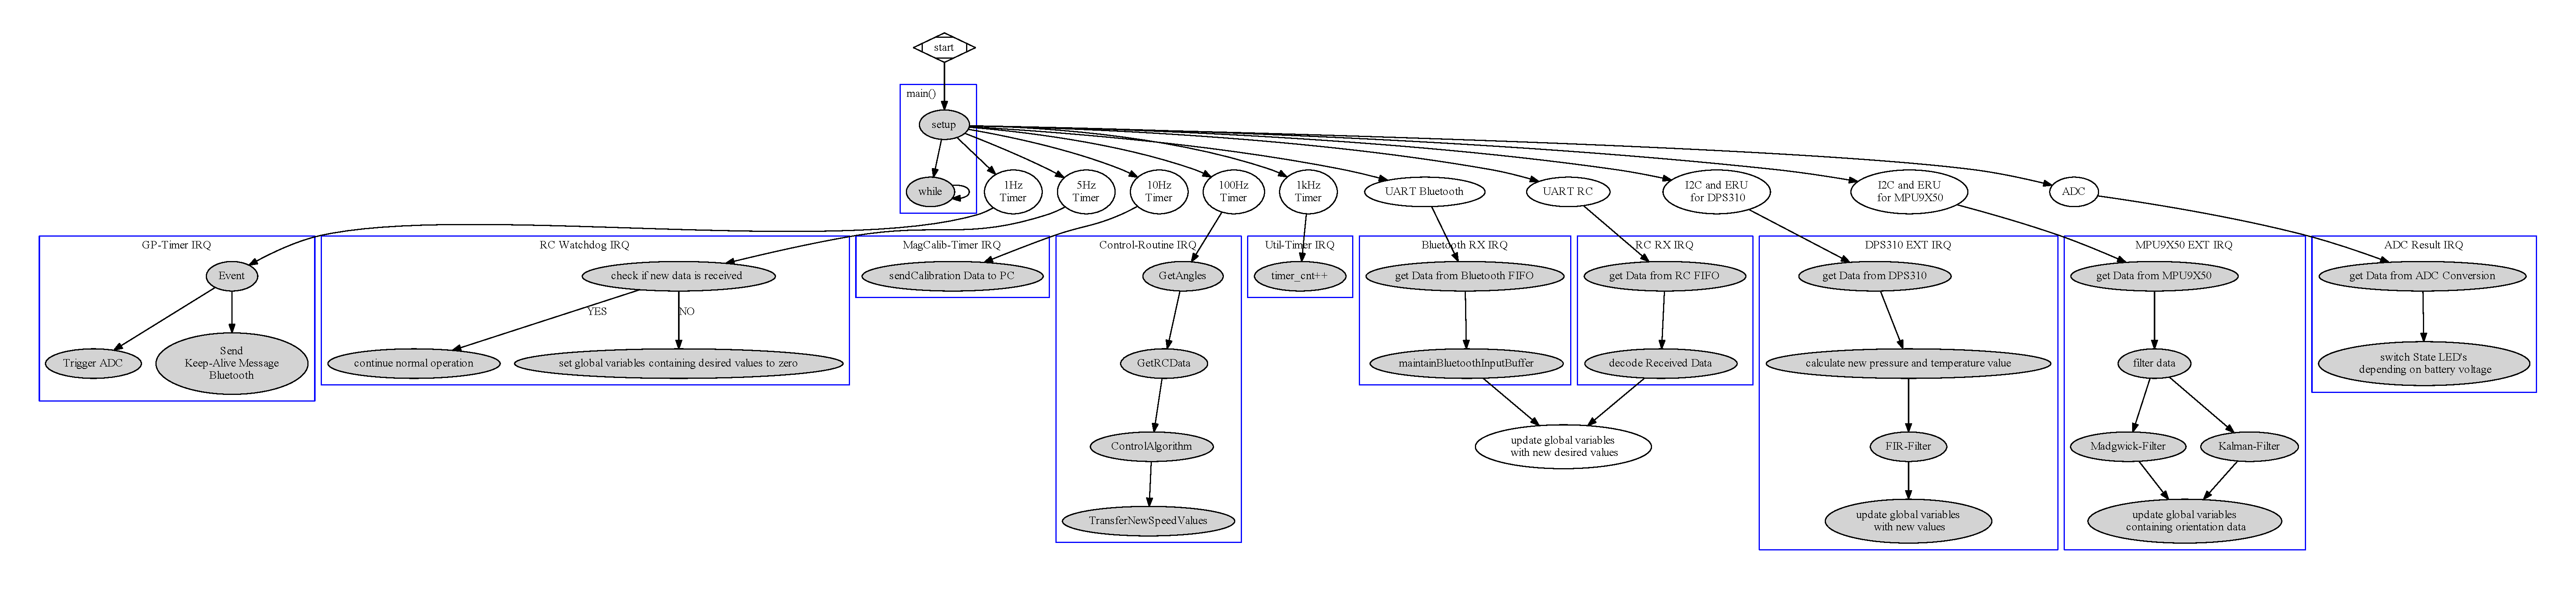
\includegraphics[width=\textwidth,height=\textheight/2,keepaspectratio=true]{dot_inline_dotgraph_1}}
\end{DoxyImageNoCaption}
 ~\newline


~\newline
 ~\newline
 ~\newline
 ~\newline
 

{\bfseries  License Terms and Copyright Information }

Copyright (c) 2015, Infineon Technologies AG All rights reserved.

Redistribution and use in source and binary forms, with or without modification, are permitted provided that the following conditions are met\+:
\begin{DoxyItemize}
\item Redistributions of source code must retain the above copyright notice, this list of conditions and the following disclaimer.
\item Redistributions in binary form must reproduce the above copyright notice, this list of conditions and the following disclaimer in the documentation and/or other materials provided with the distribution.
\item Neither the name of the copyright holders nor the names of its contributors may be used to endorse or promote products derived from this software without specific prior written permission.
\end{DoxyItemize}

T\+H\+IS S\+O\+F\+T\+W\+A\+RE IS P\+R\+O\+V\+I\+D\+ED BY T\+HE C\+O\+P\+Y\+R\+I\+G\+HT H\+O\+L\+D\+E\+RS A\+ND C\+O\+N\+T\+R\+I\+B\+U\+T\+O\+RS \char`\"{}\+A\+S I\+S\char`\"{} A\+ND A\+NY E\+X\+P\+R\+E\+SS OR I\+M\+P\+L\+I\+ED W\+A\+R\+R\+A\+N\+T\+I\+ES, I\+N\+C\+L\+U\+D\+I\+NG, B\+UT N\+OT L\+I\+M\+I\+T\+ED TO, T\+HE I\+M\+P\+L\+I\+ED W\+A\+R\+R\+A\+N\+T\+I\+ES OF M\+E\+R\+C\+H\+A\+N\+T\+A\+B\+I\+L\+I\+TY A\+ND F\+I\+T\+N\+E\+SS F\+OR A P\+A\+R\+T\+I\+C\+U\+L\+AR P\+U\+R\+P\+O\+SE A\+RE D\+I\+S\+C\+L\+A\+I\+M\+ED. IN NO E\+V\+E\+NT S\+H\+A\+LL T\+HE C\+O\+P\+Y\+R\+I\+G\+HT H\+O\+L\+D\+ER OR C\+O\+N\+T\+R\+I\+B\+U\+T\+O\+RS BE L\+I\+A\+B\+LE F\+OR A\+NY D\+I\+R\+E\+CT, I\+N\+D\+I\+R\+E\+CT, I\+N\+C\+I\+D\+E\+N\+T\+AL, S\+P\+E\+C\+I\+AL, E\+X\+E\+M\+P\+L\+A\+RY, OR C\+O\+N\+S\+E\+Q\+U\+E\+N\+T\+I\+AL D\+A\+M\+A\+G\+ES (I\+N\+C\+L\+U\+D\+I\+NG, B\+UT N\+OT L\+I\+M\+I\+T\+ED TO, P\+R\+O\+C\+U\+R\+E\+M\+E\+NT OF S\+U\+B\+S\+T\+I\+T\+U\+TE G\+O\+O\+DS OR S\+E\+R\+V\+I\+C\+ES; L\+O\+SS OF U\+SE, D\+A\+TA, OR P\+R\+O\+F\+I\+TS; OR B\+U\+S\+I\+N\+E\+SS I\+N\+T\+E\+R\+R\+U\+P\+T\+I\+ON) H\+O\+W\+E\+V\+ER C\+A\+U\+S\+ED A\+ND ON A\+NY T\+H\+E\+O\+RY OF L\+I\+A\+B\+I\+L\+I\+TY, W\+H\+E\+T\+H\+ER IN C\+O\+N\+T\+R\+A\+CT, S\+T\+R\+I\+CT L\+I\+A\+B\+I\+L\+I\+TY, OR T\+O\+RT (I\+N\+C\+L\+U\+D\+I\+NG N\+E\+G\+L\+I\+G\+E\+N\+CE OR O\+T\+H\+E\+R\+W\+I\+SE) A\+R\+I\+S\+I\+NG IN A\+NY W\+AY O\+UT OF T\+HE U\+SE OF T\+H\+IS S\+O\+F\+T\+W\+A\+RE, E\+V\+EN IF A\+D\+V\+I\+S\+ED OF T\+HE P\+O\+S\+S\+I\+B\+I\+L\+I\+TY OF S\+U\+CH D\+A\+M\+A\+GE.

To improve the quality of the software, users are encouraged to share modifications, enhancements or bug fixes with Infineon Technologies AG (\href{mailto:support@infineon.com}{\tt support@infineon.\+com}).

{\bfseries Legal Disclaimer} The information given in this document shall in no event be regarded as a guarantee of conditions or characteristics. With respect to any examples or hints given herein, any typical values stated herein and/or any information regarding the application of the device, Infineon Technologies hereby disclaims any and all warranties and liabilities of any kind, including without limitation, warranties of non-\/infringement of intellectual property rights of any third party.

{\bfseries Information} For further information on technology, delivery terms and conditions and prices, please contact the nearest Infineon Technologies Office (www.\+infineon.\+com).

{\bfseries Warnings} Due to technical requirements, components may contain dangerous substances. For information on the types in question, please contact the nearest Infineon Technologies Office. Infineon Technologies components may be used in life-\/support devices or systems only with the express written approval of Infineon Technologies, if a failure of such components can reasonably be expected to cause the failure of that life-\/support device or system or to affect the safety or effectiveness of that device or system. Life support devices or systems are intended to be implanted in the human body or to support and/or maintain and sustain and/or protect human life. If they fail, it is reasonable to assume that the health of the user or other persons may be endangered. 